%% Decision Procedure %%%%%%%%%%%%%%%%%%%%%%%%%%%%%%%%%%%%%%%%%%%%%%%%%%
\section{The BLT Decision Procedure}
\label{sec:dp}

To describe our decision procedure, we assume that we are attempting
to check whether the constraints below are satisfiable:
%
\begin{equation}
\label{eq:prob-matrix}
    \v{l} \le \mat{A} \v{x} \le \v{u}.
    \tag{P1}
\end{equation}
%
We let $n$ denote the number of free integer variables in $\v{x} \in \ZZ^n$,
and let $m$ denote the number of constrained linear forms.  The coefficients
are rational, so $\mat{A} \in \QQ^{m \times n}$ and $\v{l},\v{u} \in \QQ^m$.

Without loss of generality we assume that $n \le m$ and that $\mat{A}$ has
rank $n$ (full rank). In case the problem at hand is such that $n > m$ and/or
that $\mat{A}$ is less than full rank, one can compute a basis of the column
space, say $\mat{A}'$, that meets the requirement (cf. \cite{Cohen}, \S~2.7.1).
The new system $\v{l} \le \mat{A}' \v{y} \le \v{u}$ is equisatisfiable with
the original and solutions of the new system
determine one or more solutions of the original.

Geometrically, we can think of $\v{l}$ and $\v{u}$ as opposite corners of an
$m$-dimensional hyperrectangle defined by
%
\[ \Co := \{ \v{z} \in \RR^m  \mid  \v{l}_i \le \v{z}_i \le \v{u}_i \}. \]
%
We refer to this as the \emph{constraint set} of the problem.
Without loss of generality we may scale the rows of \eqref{eq:prob-matrix} so
that the width of $\Co$ is the same along every axis, i.e.
%
\begin{equation}
    \label{eq:cube}
    \v{u}_i - \v{l}_i = \v{u}_j - \v{l}_j \quad \forall \, i,j \in \{1,\ldots,m\}.
\end{equation}
%
Note that this transformation makes $\Co$ a \emph{hypercube}.
We let $d_\Co$ denote the common width, and let $r_\Co = d_\Co/2$ denote the
corresponding radius of the hypercube.

The problem given by \eqref{eq:prob-matrix} can also be characterized as
trying to find a common point in both a hypercube and a
lattice.
The columns of $\mat{A}$, regarded as vectors, generate a lattice.
%
Let $\{\v{b}_1, \v{b}_2, \ldots, \v{b}_n\}$ denote the column vectors of $\mat{A}$ and define:
%
\begin{equation}
    \label{eq:lattice-def}
    \La := \left\{ a_1 \v{b}_1 + \cdots + a_n \v{b}_n \in \RR^m \mid
            a_i \in \ZZ \right\}
\end{equation}
%
By our assumption that $\mat{A}$ has full rank,
$\{\v{b}_1, \ldots, \v{b}_n\}$ are linearly independent,
and there is a one-to-one
correspondance between elements in $\La \cap \Co$ and
satifying assignments to~\eqref{eq:prob-matrix}.
%
It follows that checking the satisfiability of~\eqref{eq:prob-matrix}
is equivalent to deciding whether $\La \cap \Co$ is non-empty.

The set $\La \cap \Co$ is guaranteed to be finite as a
lattice must have a finite number of elements in any space with
a bounded volume.
%
Due to the one-to-one correspondance, the number of
solutions to~\eqref{eq:prob-matrix} must be finite as well, and
hence a procedure capable of enumerating the elements in $\La \cap \Co$ can
be used as a decision procedure for checking the satisfiability
of~\eqref{eq:prob-matrix}.

Before describing such a procedure, we note that a nice feature
of the lattice and hypercube formulation is that it provides
a simple way to estimate the number of satisfying assignments. The
\emph{volume} of a lattice $\La$ can be defined in several ways (see
\cite{Lenstra}, \S5), but the simplest computationally is $\vol(\La) =
\abs{\det{\m{B}}}$ where the columns of $\m{B}$ generate $\La$. Then, the
number of elements of $\La \cap \Co$ is approximately
$\vol{\Co}\:{/}\:\vol{\La}$.
We will
use this to compute the number of expected solutions for the JPEG preimage
problems described in the Section~\ref{sec:jpeg}.

% We will lateFigure
%\ref{fig:solution_count} shows a plot of this estimate for a specific family
%of problems.


%% Decision Procedure %%%%%%%%%%%%%%%%%%%%%%%%%%%%%%%%%%%%%%%%%%%%%%%

\subsection{Enumerating Lattice Elements}
\label{ssec:dp}

% What I want to say...

% Our algorithm is a search over the tree of partial assignments $x_1 = a_1, x_2
% = a_2, \ldots, x_j = a_j$. We use a \emph{best-first} search strategy, where
% "best" at each step means making the assignment to the next variable
% such that the resulting layer is the \emph{closest} one to center among the
% remaining possibilities. The best-first search is also pruned by keeping track
% of a best known upper bound on the distance of a closest lattice vector to
% center. Layers whose distance to center exceeds the known upper bound are not
% examined.
%
% In section \ref{ssec:cvp-inf}, we discuss a slightly more general family of
% search strategies and show that they have good properties. After that we give
% some details about our implementation.
%

We now turn our attention to the problem of enumerating the elements
$\La \cap \Co$.  Recall that, without loss of generality, we have
taken $\Co$ to be a hypercube. Let $\v{p}$ denote the geometric center
of $\Co$:
%
\begin{equation}
    \label{eq:center}
    \v{p} := (\frac{\v{l}_1 + \v{u}_1}{2}, \ldots, \frac{\v{l}_m + \v{u}_m}{2}).
\end{equation}
With respect to the $\linf$ metric, $\Co$ is a closed ball of radius $r_\Co$,
centered at $\v{p}$, and hence the elements in $\La \cap \Co$ are
precisely those that are at most a distance $r_\Co$ from $\v{p}$.

Algorithms for finding lattice elements that are close to a given point have been
extensively studied and many algorithmic approaches to it exist; see
\cite{AgrellEtAl} for a good survey.
%
We have developed a complete search procedure by adapting the Schnorr-Euchner
algorithm for computing the closest vector point to a
lattice~\cite{Schnorr-Euchner}.

%In adapting the algorithm, we have made three changes: (1) We use the $\linf$
%metric instead of the Euclidean $\ltwo$
%metric; (2) rather than compute the closest element, we immediately return
%when we find an element within the hypercube; and (3) we prune search paths
%when the $R_\Co$
%Our adaption %$\linf$, both because of its performance characteristics and the ease with
%which we could change metrics.

% In particular, $\v{z} \in \Co$ if and only if $\norminf{z - p} \le r_{\Co}$.
%In the algorithm below we use \proc{Center} to denote the calculation
%\eqref{eq:center}.

%Now, suppose we have a procedure $\proc{Closest}_\infty$ which takes as input
%a lattice $\La \subset \RR^m$, a point $\v{q} \in \RR^m$, and returns a
%closest lattice vector to $\v{q}$, not in the usual $L^2$ metric, but in the
%$\linf$ metric. Assuming this for the moment, we arrive at our decision
%procedure for \eqref{eq:prob-matrix}.

%\begin{algorithm}[H]
    %\SetLine
%    \KwIn{a lattice $\La \subset \RR^m$ and a hypercube $\Co$}
%    \KwOut{``SAT'' and a $\v{z} \in \La \cap \Co$, or ``UNSAT''}
%    $\v{p} \leftarrow \proc{Center}(\Co)$\;
%    $\v{r} \leftarrow \proc{Closest}_\infty(\La, \v{p})$\;
%    \eIf{$\v{r} \in \Co$}{
%        \KwRet{$(\text{SAT}, \v{r})$}\;
%    }{
%        \KwRet{UNSAT}\;
%    }
%    \caption{Decision procedure for lattice points in a hypercube}
%\end{algorithm}

%The first branch is obviously correct. For the alternative, simply observe
%that if the closest lattice vector to $\v{p}$ in the $\linf$ metric is not
%contained in $\Co$ then there can be no lattice vector in $\Co$ (any such
%vector would be strictly closer to $\v{p}$).

%The utility of this simple procedure obviously hinges on
%$\proc{Closest}_\infty$.

%\subsection{Closest Vector Search with Infinity Norm}
%\label{ssec:cvp-inf}

%The closest vector problem has been extensively studied and many algorithmic
%approaches to it exist; see \cite{AgrellEtAl} for a good survey. In our
%implementation BLT we have chosen to adapt the Schnorr-Euchner strategy for
%$\linf$, both because of its performance characteristics and the ease with
%which we could change metrics.
\newcommand{\ruleref}{\textbf{Split}}

We model our search procedure as a non-deterministic transition rule on partial
assignments to the vectors $\v{x}$.  The procedure begins with the empty
assignment $\emptyset$, and incrementally assigns values to variables in $\v{x}$.
If the transition rule terminates with a complete assignment
$\v{u} \in \ZZ^n$, then $\v{u}$ is a solution to the constraint
problem.
%
\begin{equation}
%\label{eq:rules-split}
%\tag{\textbf{Split}}
\mathbf{(Split)}
\hspace{20pt} \theta \ \Rightarrow \ \theta \cup \{\,j \mapsto s\,\}
   \ \textbf{where}\,\begin{cases}
      j \in \{\,1, \ldots, n\,\} \setminus \fn{dom}(\theta)\\
      s \in \ZZ\ \textbf{s.t.}
      \ \La^\RR_{\theta \cup \{\,j \mapsto s\,\}} \cap \Co \neq \emptyset
      \end{cases}
\end{equation}

This rule takes a partial assignment $\theta$, and extends it with an additional
binding $j \mapsto s$ such that the real-affine linear space
$\La^\RR_{\theta \cup \{\,j \mapsto s\,\}}$ of the resulting assignment
intersects with $\Co$.  This rule models backtracking implicitly; at each
step, we may find that there is no legal value $s$ to assign $j$.  If this
occurs, our procedure must backtrack to a previous step, and explore an
alternative assignment.

We can show that the set of lattice points in $\Co$ can be enumerated by
applying~\ruleref{} transitively starting
from $\emptyset$.
%
Before stating the theorem, we first observe that each point $\v{x} \in \La$
can be expressed as the weighted sum of the columns in $\mat{A}$,
(i.e.,~$\v{x} = \mat{A}\v{u}$ for some unique $\v{u} \in \ZZ^n$).
%
\begin{thm}
  For each vector $\v{u} \in \ZZ^n$, $\mat{A} \v{u} \in \Co$ iff. there is
  a derivation $\emptyset \Rightarrow^{+} \v{u}$.
\end{thm}
\begin{proof}
%
To see that $\emptyset \Rightarrow^{+} \v{u}$ implies $\mat{A} \v{u} \in \Co$,
observe that the proceeding step must have shown that
$\La^\RR_{\v{u}} \cap \Co \neq \emptyset$.  Since $\v{u}$
is a complete assignment, $\La^\RR_{\v{u}} = \{\,\mat{A} \v{u}\,\}$, and
hence $\mat{A} \v{u} \in \Co$.

To see that $\mat{A} \v{u} \in \Co$ implies $\emptyset \Rightarrow^{+} \v{u}$,
observe that for all
partial assignments $\theta$, $\La^\RR_\theta \cap \Co \neq \emptyset$
implies that $\emptyset \Rightarrow^{+} \theta$
by induction on the number of bindings in $\theta$.
%
For a complete assignment $\v{u}$, $\La^\RR_{\v{u}} = \{\,\mat{A} \v{u}\}$.
Hence, if $\mat{A} \v{u}$ is in $\Co$, then
$\La^\RR_{\v{u}}$ is a non-empty subset of $\Co$ and $\varnothing \Rightarrow^{+} \v{u}$.
\end{proof}
%
We note that the above theorem holds regardless of the order in which we choose
the values of $j$ in~\ruleref{}.  We only need to consider all valid
assignments to $s$ once we have chosen $j$.  An implementation then has
a choice in which it can use different heuristics to search for an
assignment.
%
We will briefly describe
the heuristics used by BLT in Section~\ref{ssec:blt-optimizations}.

The previous theorem shows that the transition rule is sound and complete from
a logical point of view, to show that it is computable
we prove the following:

\begin{thm}
  The set of partial assignments $\theta$ such that
  $\emptyset \Rightarrow^{+} \theta$ is finite and
  computable.
  \label{thm:computable}
\end{thm}

\begin{proof}
As each application of~\ruleref{} adds an additional
binding to the substitution, the number of applications along any
path is bounded by $n$.  To show that the set of $\theta$ is finite,
we must show that the number of potential values of $s$ used to
instantiate~\ruleref{} is both finite and computable.
More precisely, we must prove that
there are at most a finite number of integers $s \in \ZZ$ such that
\begin{equation}
\La^\RR_{\theta \cup \{\,j \mapsto s\,\}} \cap \Co \neq \emptyset.
\label{eq:extend_theta}
\end{equation}
%
Observe that for any $u,k \in \ZZ$ with $k \neq 0$, the affine set
$\La^\RR_{\theta \cup \{\,j \mapsto u+k\,\}}$ can be
obtained by shifting the set $\La^\RR_{\theta \cup \{\,j \mapsto u\,\}}$
by a multiple $k$ of the basis vector $\v{b}_j$.  As $\v{b}_j$ is linearly
independent from the other basis vectors, it follows that
$\La^\RR_{\theta \cup \{\,j \mapsto u\,\}}$ and
$\La^\RR_{\theta \cup \{\,j \mapsto u+k\,\}}$
are disjoint and separated by some
positive distance $k \times d_{\theta,j}$ where $d_{\theta,j}$ is the distance
between the adjacent hyperplanes $\La^\RR_{\theta \cup \{\,j \mapsto 0\,\}}$ and
$\La^\RR_{\theta \cup \{\,j \mapsto 1\,\}}$
%
As the distance between any two points $\v{x}, \v{y} \in \Co$ is at most
$d_\Co$, it follows that the number of distinct $s$
satisfying~\eqref{eq:extend_theta} is at most
$d_\Co / d_{\theta,j}$.  Moreover, as both $\Co$ and
$\La^\RR_{\theta \cup \{\,j \mapsto s\,\}}$ are convex, there
must be a bounded interval $s \in \{\,l,l+1,\dots, u-1, u\,\}$
of values satisfying~\eqref{eq:extend_theta}.

Rather than compute the bounds explicitly, we
compute the $\linf$-distance between $\La^\RR_\theta$ and the point $\v{p}$ at
the center of $\Co$ using the reduction to linear programming described at the
end of the Section~\ref{sec:preliminaries} in equation~\eqref{eq:set_distance}.
%
This reduction to linear programming allows one to find an assignment
$\v{y} \in \RR^{n}$ so that $\mat{A} \v{y}$ is one of the points
in $\La^\RR_\theta$ with minimal distance to $\v{p}$.  We can then start by
considering for $s$ the points $\{\,\floor{\v{y}_j},\,\floor{\v{y}_j-1},\dots\,\}$
and $\{\,\ceil{\v{y}_j},\,\ceil{\v{y}_j+1},\dots\,\}$ until we have
explored all the assignments in the set $\{\,l,l+1,\dots, u\,\}$.
%
\end{proof}

%\proc{Split} says we can take a sublayer in $S$ and decompose it into its
%component sub-sublayers by choosing an unassigned index $j$. The assignments
%$s_i$ are taken to be precisely those for which $d_\infty(\La^\RR_{I \cup (j,
%    s_i)}, p) < r$. This is always a finite set of consecutive integers.
% See figure \ref{fig:layers} for illustration.
%
%\proc{Prune} removes sublayers that we know have no points closer to $\v{p}$
%than $r$.
%
%Finally, \proc{Satisfiable} applies to 0-dimensional sublayers, i.e. lattice
%points. If $\La_I = \{ \v{y} \}$ and the distance from $\v{y}$ to $\v{p}$ is
%less than $r_\Co$, we have found a satisfying assignment $I$.

% \begin{figure}
%     \centering
%     \vspace{0.1cm}
%     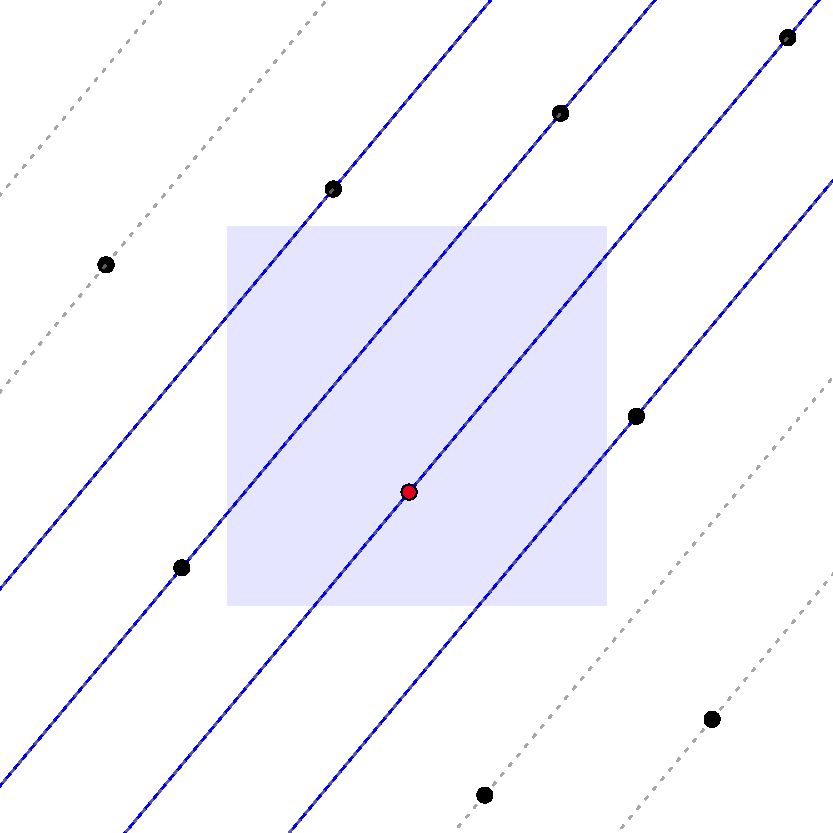
\includegraphics[width=0.48\textwidth]{lattice-layers}
%     \caption{\proc{Split} $\La_I$ into sublayers}
%     \label{fig:layers}
% \end{figure}

%Starting at some initial state $S_0$, a \emph{derivation} in this system is a
%sequence of transitions $S_0 \Rightarrow S_1 \Rightarrow \cdots$ using any of
%the three rules as long as their precondition applies. We call any state of
%the form $(\emptyset, r, \v{z})$ a final state.
%
%\begin{lem}
%    \label{lem:search}
%    The transition system described above always terminates in a final state, i.e.
%    \begin{enumerate}
%        \item every derivation is finite,
%        \item the only states in which no rule applies are final states.
%    \end{enumerate}
%\end{lem}
%
%\begin{proof}
%Consider the function $\nu$ which maps states to $n+1$-tuples of natural
%numbers: $\nu(S, r, \v{z})_i = \#\{\La_I \in S \mid \abs{I}=i \}$ for $i=0,\ldots,n$.
%We claim that all three transition rules cause $\nu$ to strictly decrease in
%the lexicographic order. For \proc{Prune} and \proc{Record} this is obvious.
%Applying $\proc{Split}_{j,I}$ causes $\nu_{\abs{I}}$ to decrease by 1 and
%$\nu_{\abs{I}+1}$ to increase (by an amount bounded above by a constant
%multiple of $r$). Hence $\nu$ strictly decreases in lexicographic order and so
%every derivation is finite.
%
%For (2), suppose to the contrary $(S, r, \v{z})$ is a state such that $S \ne
%\emptyset$ but none of the transition rules apply. Choose a $\La_I \in S$. If
%$\abs{I} < n$ then $\proc{Split}_{j,I}$ applies for some $j$. Otherwise, if
%$\abs{I} = n$ then either $d_\infty(\La^\RR_I, \v{p}) \ge r$, in which case
%$\proc{Prune}_I$ applies, or the opposite holds, in which case
%$\proc{Record}_I$ applies. Thus we have a contradiction.
%\end{proof}
%
%\begin{thm}
%    \label{thm:closest}
%    Let $\v{z}_0$ be an arbitrary lattice vector and $r_0 = d_\infty(\v{z}_0,
%    \v{p})$. Then any derivation starting with initial state
%    $(\{\La_\emptyset\}, r_0, \v{z}_0)$ terminates at a final state $(\{\},
%    r_f, \v{z}_f)$ in which $\v{z}$ is a closest vector in $\La$ to $\v{p}$.
%\end{thm}
%
%\begin{proof}
%Assume to the contrary that there is a \emph{closer} lattice vector
%$\tz$. Clearly $\tz \in \La_\emptyset = \La$. Further, if
%we are at a state $(S, r, \v{z})$ in which $\proc{Split}_{j,I}$ applies and $\tz \in
%\La_I$, then there is a new sublayer produced by $\proc{Split}$ that contains
%$\tz$. This follows from the definition of \proc{Split}, since $\tz$ is in
%\emph{some} sublayer of $\La_I$, say $\La_{I \cup (j,s)}$ and
%$d_\infty(\La^\RR_{I \cup (j,s)}, \v{p}) \le d_\infty(\tz, \v{p}) \le r$, the
%latter inequality following from our assumption that $\tz$ is closer than the
%final vector $\v{z}_f$ and hence than $\v{z}$. Similarly it should be clear
%that if at any state, $\tz \in \La_I$ and $\La_I \in S$, then $\proc{Prune}_I$
%does not apply.

%The above argument implies that at some point in our derivation, the
%$0$-dimensional sublayer $\La_J = \{ \tz \}$ must appear. The only rule that
%removes it is $\proc{Record}_J$. Hence, $d_\infty(\tz, \v{p}) \le r_f =
%d_\infty(\v{z}_f, \v{p})$, a contradiction.
%\end{proof}

% The Schnorr-Euchner strategy is best understood as a recursive
% search operation. Recall the problem is to find a $\v{z} \in \La$ such that
% $\norminf{\v{z}-\v{p}}$ is minimal.
%
%
% The main idea in the Schnorr-Euchner search strategy is to recursively search
% for a closet vector in a finite number of the layers, ordered by increasing
% distance from the target point. First we discuss which layers are searched and
% then how to compute the $\linf$ distance from the target point to a layer.
%
% Suppose for a moment that an upper bound $\rho$ is known on the distance from a
% closest vector to $\v{p}$. In this case it suffices to search a finite number
% of consecutive layers.
%
% \begin{lemma}
%     \label{lem:layers-to-search}
%     If $d(\La, p) \le \rho$ then a closest vector is contained in some layer
%     $\mathcal{Y}_a$ such that $\mathcal{Y}^\RR_a \cap H \ne \emptyset$ and
%     moreover $\{ a \in \ZZ \mid \mathcal{Y}^\RR_a \cap H \ne \emptyset \}$ is
%     bounded set of consecutive integers.
% \end{lemma}
% \begin{proof}
%     TODO
% \end{proof}
% The order in which layers are searched makes a significant difference in
% practice. We discuss the choice our implementation makes at the end of the
% section.

\subsection{Implementation Decisions}
\label{ssec:blt-optimizations}

Turning the previous section into a working and efficient
procedure involves many more choices and details than
we have room to describe.  We would like to indicate, however a couple choices
we have made in implementing BLT.

\textbf{Search Strategy.}
%
In implementing the transition system,
we have chosen to adopt a strategy similar to Schnorr and Euchner
in~\cite{Schnorr-Euchner}.
%
We use the LLL algorithm~\cite{Lenstra} to generate a reduced basis, and
fix the basis vectors by sorting in order of decreasing $L^2$ magnitude.
%
We then proceed by applying \ruleref{} in a depth first order
with the sequence of $j$'s chosen according to our basis order.
%
The variables with the largest magnitude are typically the
most-constrained variables in our problems, as they have the largest
distance between adjacent sublayers.
%
Choosing the most constrained variable is a common strategy in
constraint satisfication, and we have found the strategy effective
in this case as well.

The other choice we have with split is to consider which values of $s$ to
explore.  To maximize the likelihood of finding a satisfying assignment,
we would like to choose a value for $s$ that imposes the least
constraints on subsequent assignments.
This could be done by choosing
an assignment to $s$ that maximizes the volume of the intersection
between the hypercube $\Co$ and real-affine set
$\La^\RR_{\theta \cup \{\,j \mapsto s\,\}}$.

Unfortunately, we do not know of an efficient way to compute the
$s$ with the maximal volume\footnote{In~\cite{dyer_freize88}, the
authors show that the related problem of computing the volume of the
intersection of the unit cube and a rational halfspace is \#P-hard.},
but we have developed a proxy that works well in practice.
%
As alluded to in the proof of Theorem~\ref{thm:computable}, we
use linear programming to find an initial assignment to $s$ that minimizes
the $\linf$-distance between the center of the hypercube $\v{p}$ and
$\La^\RR_{\theta \cup \{\,j \mapsto s\,\}}$.
%
Since the distance between the sublayer and center point is minimal, we
can expect that the volume of the sublayer within the hypercube should
be maximal or near maximal.  If this assignment is found
infeasible, and we backtrack, then we explore adjacent assignments
$s + \delta, s - \delta, s + 2\delta, \ldots{}$, where $\delta = \pm 1$
depending on orientation, in order of increasing distance.

%In implementing the transition system,
%we have chosen to adopt a strategy similar to Schnorr and Euchner in
%\cite{Schnorr-Euchner}. After choosing a lattice basis, we fix an ordering of
%the basis vectors and proceed by applying $\proc{Split}_{j,-}$ for the
%sequence of $j$'s corresponding to our basis order. After splitting say
%$\La_I$ into $\La_{I \cup (i,a_1)}, \ldots, \La_{I \cup (i,a_k)}$ we choose
%the sublayer among these that is closest to $\v{p}$ and apply \proc{Split}
%there.  Thus we have a best-first search that always follows the closest
%sublayer first. In this way we quickly reach a $0$-dimensional sublayer,
%namely a lattice point, and apply \proc{Record}. This point is known as the
%\emph{Babai point} in the literature and gives us a good starting $r$ and
%$\v{z}$ value for our state.

%After reaching the Babai point, we backtrack to the $1$-dimensional layer it
%came from and decide to either \proc{Prune} or \proc{Record} at the other
%sublayers there, doing so in order of increasing distance from $\v{p}$
%\footnote{If the closest sublayer was $\La_{I \cup (j,s)}$ and $\v{p}$ is
%``above'' it with respect to the direction of $\v{v}_j$, then one can show
%that the assignments $(s_i) = (s, s+1, s-1, s+2, \ldots)$ enumerate the
%sublayers in order of increasing distance from $\v{p}$.}.  The advantage
%of making this choice is that when we hit a sublayer that \proc{Prune} applies
%to, then we infer that all the other sublayers at this level can be pruned and
%we jump up another level.

%Our implementation deviates slightly from the transition system
%described here in order to make some crucial optimizations. When solving a
%bounded integer constraint problem, the goal is to find a lattice vector
%satisfying the constraints. Accordingly, in our $\proc{Closest}_\infty$
%implementation we check at each application of \proc{Record} whether the new
%point satisfies the constraints and if it does we return early as there is no
%need to find the closest solution. In the problems we've studied, early exit
%like this saves an enormous amount of time, in particular when the Babai point
%mentioned above already satisfies the constraints.

%Finally, note that we've described $\proc{Closest}_\infty$ as starting with
%the state $(\La_\emptyset, r_0, \v{z}_0)$ for some $\v{z}_0 \in \La$ and $r_0 =
%d_\infty(\v{z}_0, \v{p})$. However, if our constraint set $\Co$ is a hypercube
%with radius $r_\Co$, it's obviously better to start with $r_0 = r_\Co$ as this
%is likely to be a much tighter upper bound. Some of the arguments above need
%to be modified to account for this, but the performance gain is significant.

% \paragraph{Lattice Basis.} In section \ref{sec:bcp} we hinted
% choosing a good lattice basis to work with is important. For solving the
% problems presented in section \ref{sec:jpeg}, it is essential. As a
% pre-processing step in BLT we compute a reduced lattice basis once and for all
% using Algorithm 2.6.3 of \cite{Cohen} as implemented in \cite{NTL}. This is
% done \emph{after} the hypercube scaling since, depending on the nature of the constraints
% present, this step can make the lattice matrix quite non-orthogonal.

%Joe
\textbf{Layer-point distance.}
%
Due to efficiency concerns as well as implementation issues with linking
GMP with other Haskell code that BLT is linked against,
we compute the distance using a conventional linear programming solver,
GLPK \cite{GLPK}, which uses IEEE double precision floating point for
its calculations.  If the distance calculation is inaccurate, there is the
potential to prune a sublayer that is mistaken for being slightly too far
away,
and consequently BLT may incorrectly return UNSAT.  In cases where it
returns SAT, the model is checked against the problem for certainty. In
principle the distance calculations can be done using exact
arithmetic\footnote{GLPK supports this directly.} or arbitrary-precision
floating point arithmetic, but we have not attempted to do so yet.
